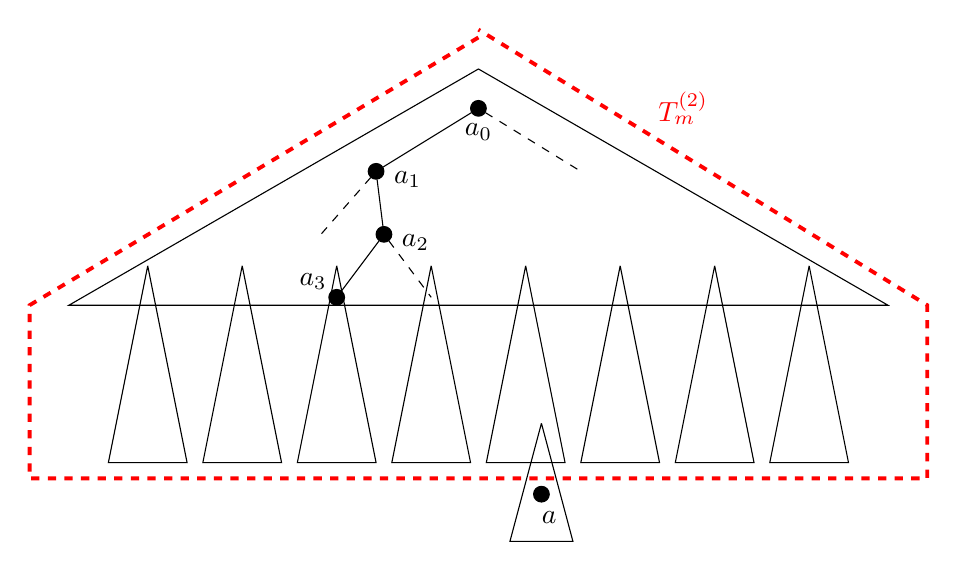
\begin{tikzpicture}

% TRIANGLES %%%%%%%%%%%%%%%%%%%%%%%%%%%%%%%%%%%%%%%%%%%%%%%%%%%%%%%%%%%%%%%%%%
%Layer0
\draw [color = black] (6.2,7.5) -- (1.0,4.5) -- (11.4,4.5) -- (6.2,7.5);

%layer1
\draw [color = black] (2.0,5.0) -- (1.5,2.5) -- (2.5,2.5) -- (2.0,5.0);
\draw [color = black] (3.2,5.0) -- (2.7,2.5) -- (3.7,2.5) -- (3.2,5.0);
\draw [color = black] (4.4,5.0) -- (3.9,2.5) -- (4.9,2.5) -- (4.4,5.0);
\draw [color = black] (5.6,5.0) -- (5.1,2.5) -- (6.1,2.5) -- (5.6,5.0);
\draw [color = black] (6.8,5.0) -- (6.3,2.5) -- (7.3,2.5) -- (6.8,5.0);
\draw [color = black] (8.0,5.0) -- (7.5,2.5) -- (8.5,2.5) -- (8.0,5.0);
\draw [color = black] (9.2,5.0) -- (8.7,2.5) -- (9.7,2.5) -- (9.2,5.0);
\draw [color = black] (10.4,5.0) -- (9.9,2.5) -- (10.9,2.5) -- (10.4,5.0);

%layer2
\draw [color = black] (7.0,3.0) -- (6.6,1.5) -- (7.4,1.5) -- (7.0,3.0);

%red
\draw [color = red, line width = 1.4pt, dashed] (6.2,7.9) -- (0.5,4.5) -- (0.5,2.3) -- (11.9,2.3) -- (11.9,4.5) -- (6.2,8.0);

% NODES

\node[draw, circle, fill=black, scale=0.6] (a0) at (6.2,7.0) {};
\node[draw, circle, fill=black, scale=0.6] (a1) at (4.9,6.2) {};
\node[draw, circle, fill=black, scale=0.6] (a2) at (5.0,5.4) {};
\node[draw, circle, fill=black, scale=0.6] (a3) at (4.4,4.6) {};
\node[draw, circle, fill=black, scale=0.6] (a) at (7.0,2.1) {};

\draw (a0) -- (a1);
\draw[dashed] (a0) -- (7.5,6.2);
\draw (a1) -- (a2);
\draw[dashed] (a1) -- (4.2,5.4);
\draw (a2) -- (a3);
\draw[dashed] (a2) -- (5.6,4.6);

% ETIQUETTES

\node[color = red] at (8.8,7.0) {$T_m^{(2)}$};

\node at (6.2,6.7) {$a_0$};
\node at (5.3,6.1) {$a_1$};
\node at (5.4,5.3) {$a_2$};
\node at (4.1,4.8) {$a_3$};
\node at (7.1,1.8) {$a$};


\end{tikzpicture}
